\section{Backlog/roadmap du sprint Release Candidate}

L’objectif de ce sprint est de donner bien plus de valeur à l'utilisateur par l’ajout 
de nombreuses fonctionnalités supplémentaires. Un objectif secondaire a été l'amélioration 
de l’interface d’un point de vue visuel et pour en faciliter la compréhension. 

Pour ce faire le backlog suivant a été "embarqué" dans cette version et a résulté en la roadmap suivante:

\begin{center}
    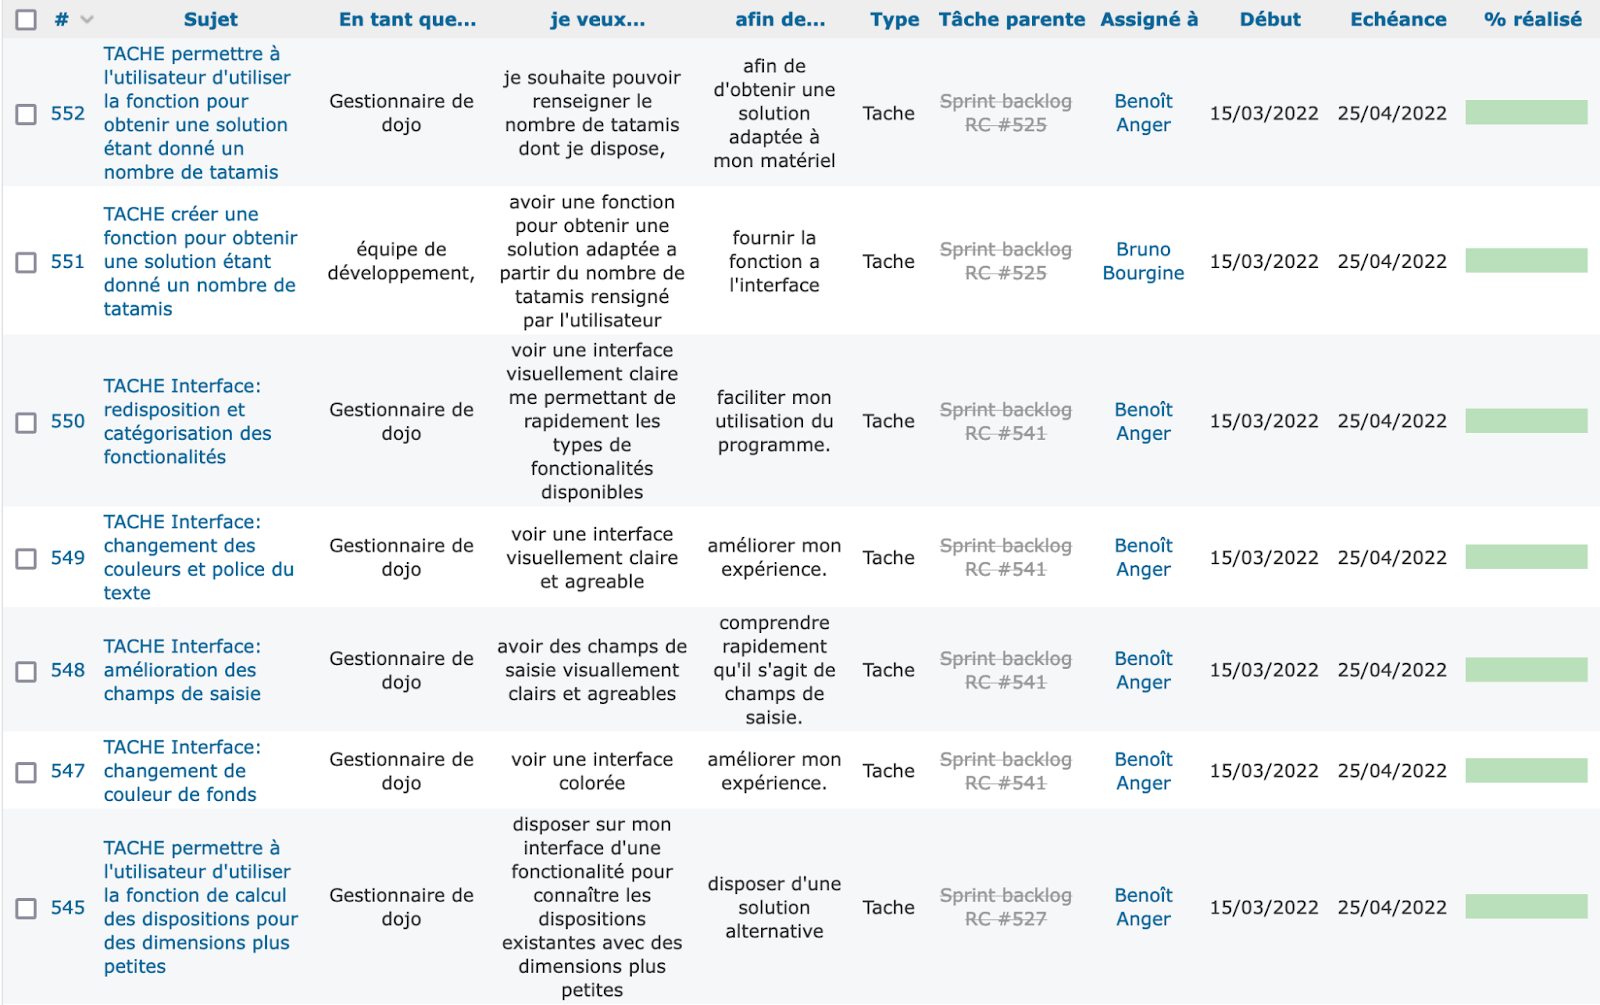
\includegraphics[width=17cm]{images/roadmap-rc-part1.png}
\end{center}

\begin{center}
    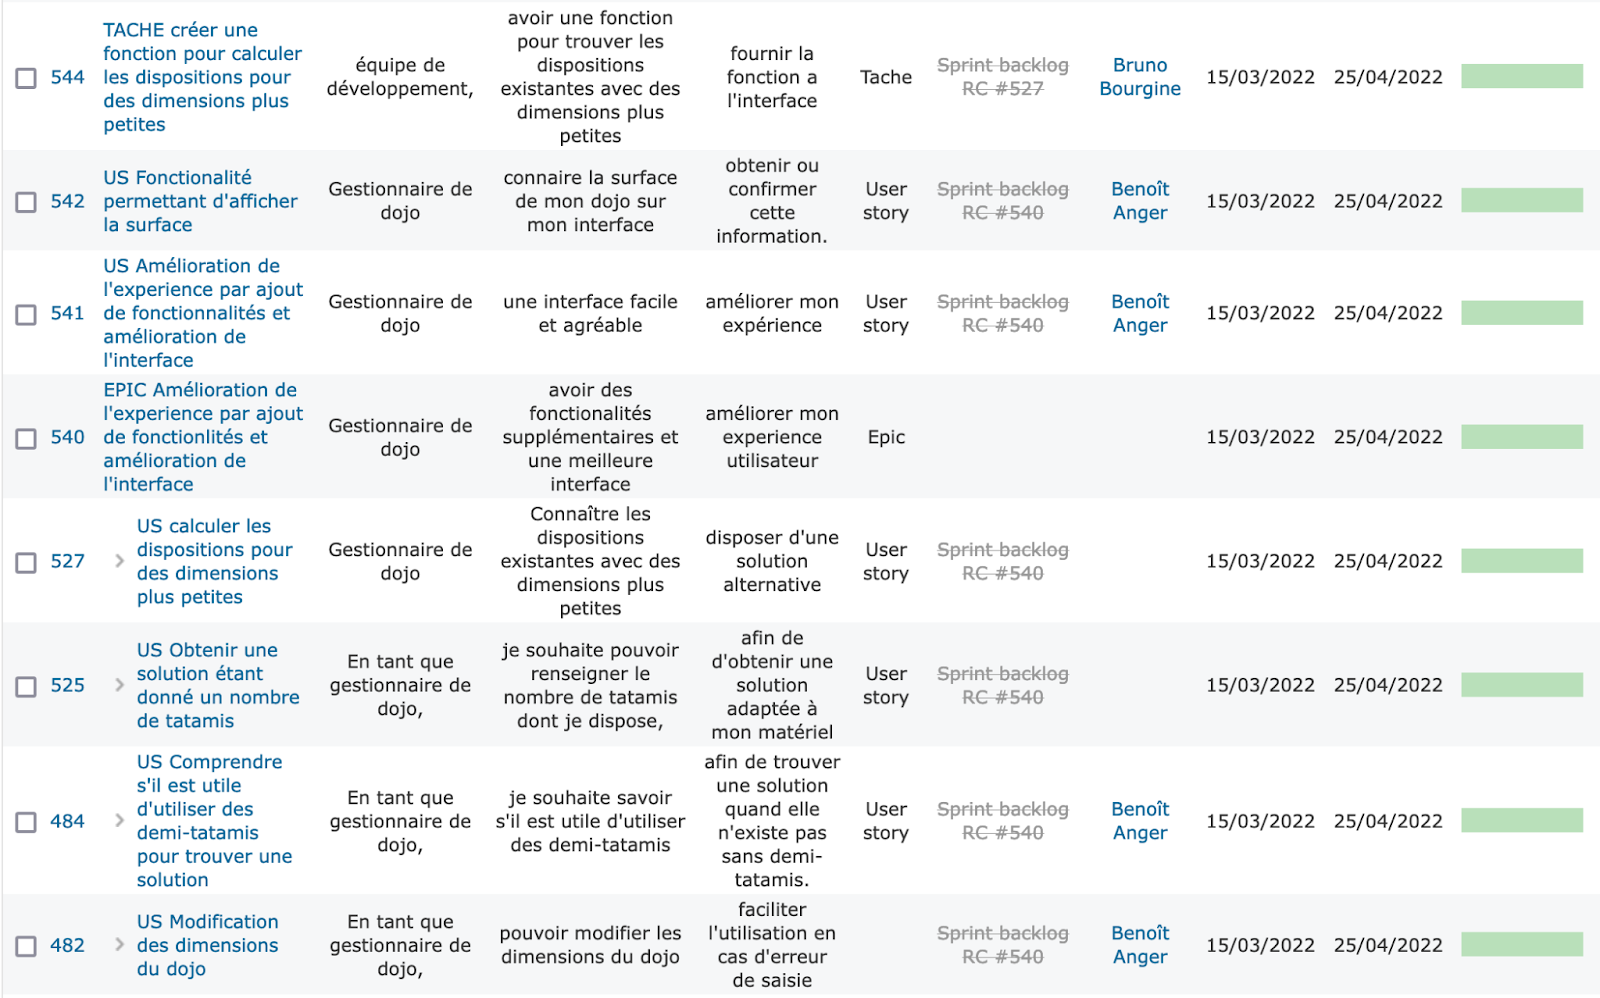
\includegraphics[width=17cm]{images/roadmap-rc-part2.png}

    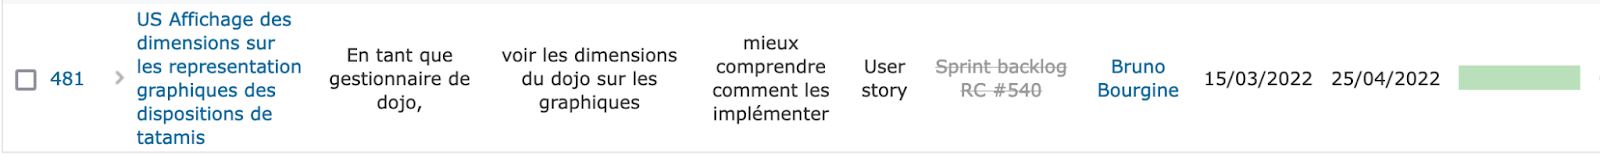
\includegraphics[width=17cm]{images/roadmap-rc-part3.png}
\end{center}


Et ici présenté en diagramme de Gantt:
\begin{center}
    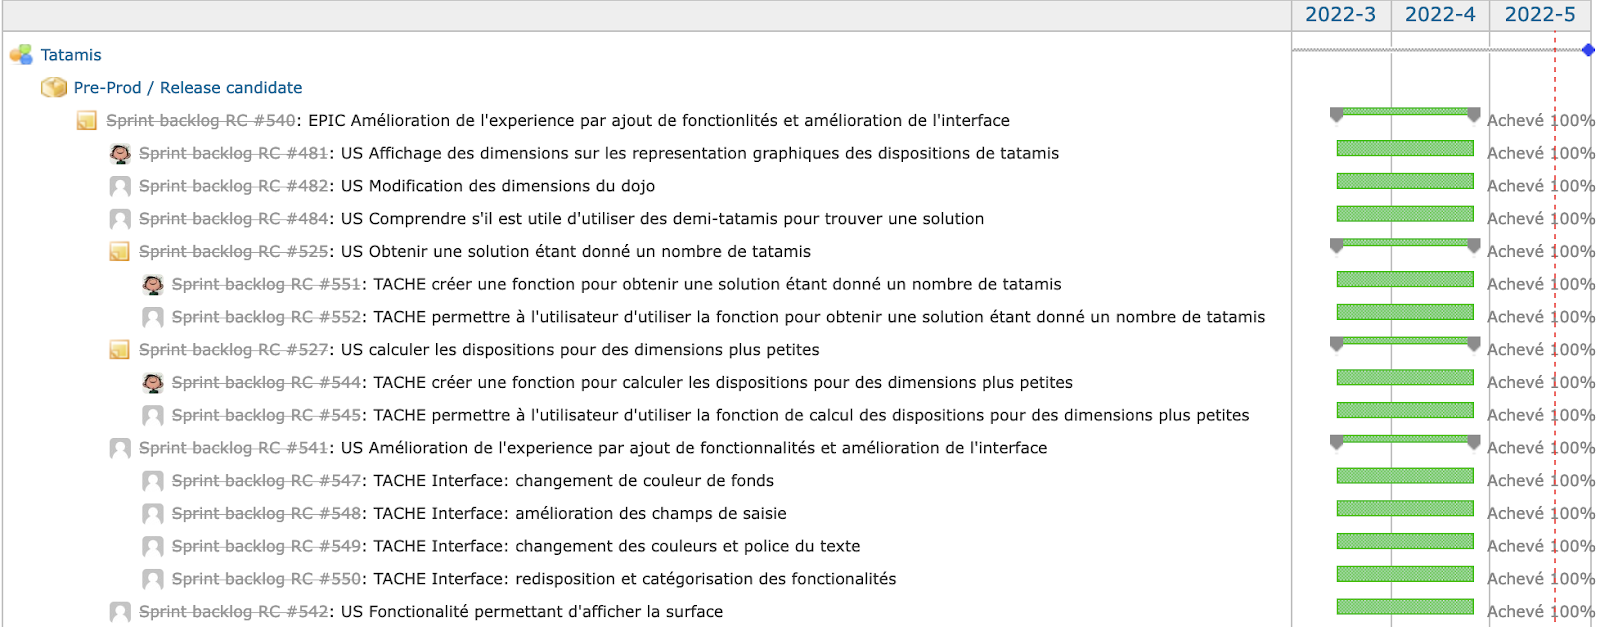
\includegraphics[width=16cm]{images/tatamis-gantt-rc.png}

\end{center}

\newpage
\section{Tests}


\noindent%
\begin{adjustwidth}{-1.5cm}{0cm}

    \renewcommand{\arraystretch}{1.2}
    {\setlength{\tabcolsep}{1.5 mm}
        \begin{testtabular}{|m{0.6cm}|m{5.5cm}|m{8cm}|m{2cm}|c|} \hline
            \rowcolor{tssteelblue} \textcolor{white}{id}                        & \textcolor{white}{Sujet}                                                                   & \textcolor{white}{Test d'acceptance (en gris : test utilisateur)}                                                                                            & \textcolor{white}{Méthode de test} & \textcolor{white}{Résultat} \\ \hline
            540 & EPIC Amélioration de l'expérience par ajout de fonctionnalités et amélioration de l'interface                      & \cellcolor{tsgrey}cf tests utilisateur des US                                                                                                                                                                                                        & Manuel          & OK       \\ \hline
            481 & US Affichage des dimensions sur les représentation graphiques des dispositions de tatamis                          & L'affichage graphique des solutions comprend un rappel des dimensions du dojo.                                                                                                                                                     & Manuel          & OK       \\ \hline
            482 & US Modification des dimensions du dojo                                                                             & L'application permet de saisir d'autres dimensions que celles initialement renseignées.                                                                                                                                            & Manuel          & OK       \\ \hline
            482 & US Modification des dimensions du dojo                                                                             & L'application permet de saisir d'autres dimensions que celles initialement renseignées.                                                                                                                                            & Manuel          & OK       \\ \hline
            484 & US Comprendre s'il est utile d'utiliser des demi-tatamis pour trouver une solution                                 & Si il n'existe pas de solutions avec des tatamis entiers, l'application affiche qu'il est toujours possible d'obtenir une solutions avec des demi-tatamis.                                                                         & Manuel          & OK       \\ \hline
            525 & US Obtenir une solution étant donné un nombre de tatamis                                                           & Lorsque l'utilisateur entre un nombre de tatamis, l'application propose une solution dont une des dimensions ne peut-être inférieure à 3 et dont le rapport largeur/longueur ne peut être inférieur à 1/3.& Manuel          & OK       \\ \hline
            551 & TACHE créer une fonction pour obtenir une solution étant donné un nombre de tatamis                                & Lorsque l'utilisateur entre un nombre de tatamis, l'application propose une solution dont une des dimensions ne peut-être inférieure à 3 et dont le rapport largeur/longueur ne peut être inférieur à 1/3.                         & Manuel          & OK       \\ \hline
            552 & TACHE permettre à l'utilisateur d'utiliser la fonction pour obtenir une solution étant donné un nombre de tatamis  & \cellcolor{tsgrey}La fonctionnalité est disponible sur l'interface utilisateur                                                                                                                                                                       & Manuel          & OK       \\ \hline
            527 & US calculer les dispositions pour des dimensions plus petites                                                      & \cellcolor{tsgrey} Lorsque l'utilisateur propose des dimensions, il n'existe pas de disposition aux dimensions plus grandes entre la(les) solution(s) alternative(s) proposée(s) par l'application et la demande de l'utilisateur. & Manuel          & OK       \\ \hline
            544 & TACHE créer une fonction pour calculer les dispositions pour des dimensions plus petites                           & Lorsque l'utilisateur propose des dimensions, il n'existe pas de disposition aux dimensions plus grandes entre la(les) solution(s) alternative(s) proposée(s) par l'application et la demande de l'utilisateur.                    & Automatisé      & OK       \\ \hline
            545 & TACHE permettre à l'utilisateur d'utiliser la fonction de calcul des dispositions pour des dimensions plus petites & \cellcolor{tsgrey}La fonctionnalité est disponible sur l'interface utilisateur                                                                                                                                                                       & Manuel          & OK       \\ \hline
            541 & US Amélioration de l'expérience par ajout de fonctionnalités et amélioration de l'interface                        & \cellcolor{tsgrey}Chaque interaction proposée par l'interface correspond à une fonctionnalité bien définie et identifiable, l'interface est intuitive est agréable visuellement.                                                                     & Manuel          & OK       \\ \hline
            547 & TACHE Interface: changement de couleur de fonds                                                                    & \cellcolor{tsgrey}Test utilisateur: Le fonds de l'interface est coloré& Manuel          & OK       \\ \hline
            548 & TACHE Interface: amélioration des champs de saisie                                                                 & \cellcolor{tsgrey}Les champs de saisie sont bien identifiables& Manuel          & OK       \\ \hline
            549 & TACHE Interface: changement des couleurs et police du texte                                                        & \cellcolor{tsgrey} Le texte est coloré et avec une police lisible et moderne& Manuel          & OK       \\ \hline
            550 & TACHE Interface: redisposition et catégorisation des fonctionnalités                                               & \cellcolor{tsgrey}Les fonctionnalités sont groupées par theme sur l'interface"& Manuel          & OK       \\ \hline
            542 & US Afficher la surface                                                                                             & \cellcolor{tsgrey} La valeur d'aire affichée sur l'interface correspond à l'aire de la surface occupée par les tatamis.& Manuel          & OK       \\ \hline
        \end{testtabular}}
\end{adjustwidth}


\section{Documentation utilisateur Release Candidate}

\subsection{Prérequis}

Configuration et installations requises:

\begin{itemize}
    \item Python 3.9 ou supérieur
    \item Librairies Python: datetime, numpy, PyQt5.QtCore, PyQt5.QtGui, PyQt5.QtWidgets, sys, time. 
    \item Installer les polices Nexa (light et bold) (fichiers otf fournis)
\end{itemize}


\subsection{Comment trouver la surface du dojo?}


\begin{enumerate}
    \item Lancer l’interface (dans le Terminal avec la ligne de commande: \texttt{python3 interface.py})
    \item Entrer dans l’interface la longueur et la largeur du dojo dans les champs prévus à cet effet.
    (Champs au bas de l’interface intitulés “Longueur (entre 1 et 25)” et “Largeur (entre 1 et 25)”). 

          \emph{Nb:
              \begin{itemize}
                  \item Vous pouvez inverser la longueur et la largeur, cela n’a pas d’importance
                  \item Vous pouvez entrer un nombre de tatamis compris entre 1 et 25.
              \end{itemize}
          }
    \item Cliquer sur le bouton: “Afficher la surface du dojo”
          \emph{ Nb: Si vous oubliez d’entrer une dimension ou si vous entrez une dimension 0,
              un message d’erreur “Erreur de saisie des dimensions. Aucune dimension ne peut avoir une valeur nulle ou vide” apparaît.}
    \item Interpréter la réponse:
          \begin{enumerate}
              \item  \textbf{Réponse}: “La surface du dojo est [Nombre]”.
                    \textbf{Interprétation}: la surface du dojo est de [Nombre] 
                    (unité identique à celle des dimensions entrées).

          \end{enumerate}
\end{enumerate}


\subsection{Comment trouver le nombre de tatamis nécessaires pour remplir un dojo?}


\begin{enumerate}
    \item Lancer l’interface (dans le Terminal avec la ligne de commande: \texttt{python3 interface.py})
    \item Entrer dans l’interface la longueur et la largeur du dojo dans les champs prévus à cet effet.
    (Champs au bas de l’interface intitulés “Longueur (entre 1 et 25)” et “Largeur (entre 1 et 25)”).

          \emph{Nb:
              \begin{itemize}
                  \item Vous pouvez inverser la longueur et la largeur, cela n’a pas d’importance
                  \item Vous pouvez entrer un nombre de tatamis compris entre 1 et 25.
              \end{itemize}
          }
    \item Cliquer sur le bouton: “Connaître le nombre de tatamis 2 $\times$ 1 nécessaires pour la taille du dojo”
          \emph{ Nb: Si vous oubliez d’entrer une dimension ou si vous entrez une dimension 0,
              un message d’erreur “Erreur de saisie des dimensions. Aucune dimension ne peut avoir une valeur nulle ou vide” apparaît.}
    \item Interpréter la réponse:
          \begin{enumerate}
              \item  \textbf{Réponse}: “Le nombre de tatamis 2x1 nécessaires pour ce dojo est : [Nombre]”.
                    \textbf{Interprétation}: il existe au moins une disposition possible et vous aurez besoin d’exactement [Nombre] tatamis pour remplir le dojo.
              \item  \textbf{Réponse}: “Demande impossible. Il n'existe pas de disposition possible avec des tatamis 2x1 pour ce dojo”. \textbf{Interprétation}:
                    il n’existe aucune disposition possible de tatamis 2 x 1 pour remplir le dojo.
          \end{enumerate}
\end{enumerate}


\subsection{Comment savoir s’il existe une disposition possible de tatamis pour un dojo donné?}


\begin{enumerate}
    \item Lancer l’interface (dans le Terminal avec la ligne de commande: \texttt{python3 interface.py})
    \item Entrer dans l’interface la longueur et la largeur du dojo dans les champs prévus à cet effet.
    (Champs au bas de l’interface intitulés “Longueur (entre 1 et 25)” et “Largeur (entre 1 et 25)”).
          \emph{Nb:
              \begin{itemize}
                  \item Vous pouvez inverser la longueur et la largeur, cela n’a pas d’importance
                  \item Vous pouvez entrer un nombre de tatamis compris entre 1 et 25.
              \end{itemize}
          }
    \item Cliquer sur le bouton: “Savoir s’il existe une disposition pour le dojo”

          \emph{Nb: Si vous oubliez d’entrer une dimension ou si vous entrez une dimension 0,
              un message d’erreur “Erreur de saisie des dimensions.
              Aucune dimension ne peut avoir une valeur nulle ou vide” apparaît.}
    \item Interpréter la réponse:
          \begin{enumerate}
              \item \textbf{Réponse}: “Il existe au moins une disposition avec des tatamis 2x1 pour ce dojo”.
                    \textbf{Interprétation}: il existe au moins une disposition possible.
              \item \textbf{Réponse}: “Il n’existe pas de disposition possible avec des tatamis 2x1 pour ce dojo”.
                    \textbf{Interprétation}: il n’existe aucune disposition possible de tatamis 2 x 1 pour remplir le dojo.
                    Il est dans ce cas probable de devoir utiliser des demi-tatamis pour remplir pleinement le dojo.
          \end{enumerate}

\end{enumerate}

\subsection{Comment savoir combien il existe de dispositions possibles de tatamis pour un dojo donné?}

\begin{enumerate}
    \item Lancer l’interface (dans le Terminal avec la ligne de commande: \texttt{python3 interface.py})
    \item Entrer dans l’interface la longueur et la largeur du dojo dans les champs prévus à cet effet.
    (Champs au bas de l’interface intitulés “Longueur (entre 1 et 25)” et “Largeur (entre 1 et 25)”). 
          \emph{Nb:
              \begin{itemize}
                  \item Vous pouvez inverser la longueur et la largeur, cela n’a pas d’importance
                  \item Vous pouvez entrer un nombre de tatamis compris entre 1 et 25.
              \end{itemize}
          }
    \item Cliquer sur le bouton: “Connaître le nombre dispositions possibles”.

          \emph{Nb: Si vous oubliez d’entrer une dimension ou si vous entrez une dimension 0,
              un message d’erreur “Erreur de saisie des dimensions.
              Aucune dimension ne peut avoir une valeur nulle ou vide” apparaît.
          }
    \item Interpréter la réponse:
          \begin{enumerate}
              \item \textbf{Réponse}: “Il existe [Nombre] dispositions possibles”.
                    \textbf{Interprétation} : il existe des dispositions pour ce dojo et [Nombre] est
                    le nombre de dispositions possibles pour remplir le dojo.
              \item \textbf{Réponse}: “Il existe 0 disposition possible”.
                    \textbf{Interprétation}: la demande est non pertinente car il n’existe pas de disposition possible
                    de tatamis 2x1 pour les dimensions du dojo.
          \end{enumerate}
\end{enumerate}


\subsection{Comment afficher une disposition?}

\begin{enumerate}
    \item Lancer l’interface (dans le Terminal avec la ligne de commande: \texttt{python3 interface.py})
    \item Entrer dans l’interface la longueur et la largeur du dojo dans les champs prévus à cet effet.
    (Champs au bas de l’interface intitulés “Longueur (entre 1 et 25)” et “Largeur (entre 1 et 25)”). 

          \emph{Nb:
              \begin{itemize}
                  \item Vous pouvez inverser la longueur et la largeur, cela n’a pas d’importance
                  \item Vous pouvez entrer un nombre de tatamis compris entre 1 et 25.
              \end{itemize}
          }
    \item Cliquer sur le bouton: “Afficher une disposition”

          \emph{Nb: Si vous oubliez d’entrer une dimension ou si vous entrez une dimension 0,
              un message d’erreur “Erreur de saisie des dimensions.
              Aucune dimension ne peut avoir une valeur nulle ou vide” apparaît.
          }

    \item Une disposition s’affiche ainsi que le rappel des dimensions du dojo, sa surface et le nombre 
    de tatamis nécessaires pour le remplir.

          Ou bien le message d’erreur suivant s’affiche: “Demande impossible.
          Il n'existe pas de disposition possible avec des tatamis 2x1 pour ce dojo” apparaît,
          ce qui signifie que la demande est non pertinente car il n’existe pas de disposition
          possible de tatamis 2x1 pour les dimensions du dojo.

\end{enumerate}

\subsection{Comment afficher toutes les dispositions possibles?}

\begin{enumerate}
    \item Lancer l’interface (dans le Terminal avec la ligne de commande: \texttt{python3 interface.py})
    \item Entrer dans l’interface la longueur et la largeur du dojo dans les champs prévus à cet effet.
    (Champs au bas de l’interface intitulés “Longueur (entre 1 et 25)” et “Largeur (entre 1 et 25)”). 

          \emph{Nb:
              \begin{itemize}
                  \item Vous pouvez inverser la longueur et la largeur, cela n’a pas d’importance
                  \item Vous pouvez entrer un nombre de tatamis compris entre 1 et 25.
              \end{itemize}
          }
    \item Cliquer sur le bouton: “Afficher toutes les dispositions possibles”

          \emph{Nb: Si vous oubliez d’entrer une dimension ou si vous entrez une dimension 0,
              un message d’erreur “Erreur de saisie des dimensions.
              Aucune dimension ne peut avoir une valeur nulle ou vide” apparaît.
          }

    \item Toutes les dispositions possibles s’affichent ainsi que le rappel des dimensions du dojo, 
    sa surface et le nombre de tatamis nécessaires pour le remplir.

          Ou bien le message d’erreur suivant s’affiche: “Demande impossible.
          Il n'existe pas de disposition possible avec des tatamis 2x1 pour ce dojo” apparaît,
          ce qui signifie que la demande est non pertinente car il n’existe pas de disposition
          possible de tatamis 2x1 pour les dimensions du dojo.

\end{enumerate}

\subsection{En cas d’absence de solutions, comment connaître la taille maximum du dojo qui permettrait de trouver au moins un disposition?}

\begin{enumerate}
    \item Lancer l’interface (dans le Terminal avec la ligne de commande: \texttt{python3 interface.py})
    \item Entrer dans l’interface la longueur et la largeur du dojo dans les champs prévus à cet effet.
    (Champs au bas de l’interface intitulés “Longueur (entre 1 et 25)” et “Largeur (entre 1 et 25)”). 

          \emph{Nb:
              \begin{itemize}
                  \item Vous pouvez inverser la longueur et la largeur, cela n’a pas d’importance
                  \item Vous pouvez entrer un nombre de tatamis compris entre 1 et 25.
              \end{itemize}
          }
    \item Cliquer sur le bouton: “Quelle taille maximum de dojo pour avoir une solution”

          \emph{Nb: Si vous oubliez d’entrer une dimension ou si vous entrez une dimension 0,
              un message d’erreur “Erreur de saisie des dimensions.
              Aucune dimension ne peut avoir une valeur nulle ou vide” apparaît.
          }

    \item Interpréter la réponse :
    \begin{enumerate}
        \item \textbf{Réponse}: “Taille maximum de dojo pour le remplir de tatamis 2 x 1. 
        La taille maximale est ([Longueur], [Largeur])”. \textbf{Interprétation}: La taille (plus petite 
        que les dimensions entrées) maximale d’un dojo pour obtenir une solution est de longueur [Longueur] et de largeur [Largeur].
        \item \textbf{Réponse}: “Demande impossible. Il existe au moins une disposition possible avec des tatamis 2x1 pour ce dojo”. 
        \textbf{Interprétation}: la demande est non pertinente car il existe au moins une disposition possible de tatamis 2x1 pour 
        les dimensions du dojo entrées. 
    \end{enumerate}
         
\end{enumerate}

\subsection{En cas d’absence de solutions, existe-t-il une solution avec des demi-tatamis?}


\begin{enumerate}
    \item Lancer l’interface (dans le Terminal avec la ligne de commande: \texttt{python3 interface.py})
    \item Entrer dans l’interface la longueur et la largeur du dojo dans les champs prévus à cet effet.
    (Champs au bas de l’interface intitulés “Longueur (entre 1 et 25)” et “Largeur (entre 1 et 25)”). 

          \emph{Nb:
              \begin{itemize}
                  \item Vous pouvez inverser la longueur et la largeur, cela n’a pas d’importance
                  \item Vous pouvez entrer un nombre de tatamis compris entre 1 et 25.
              \end{itemize}
          }
    \item Cliquer sur le bouton: “Quelle taille maximum de dojo pour avoir une solution”

          \emph{Nb: Si vous oubliez d’entrer une dimension ou si vous entrez une dimension 0,
              un message d’erreur “Erreur de saisie des dimensions.
              Aucune dimension ne peut avoir une valeur nulle ou vide” apparaît.
          }

    \item Interpréter la réponse :
    \begin{enumerate}
        \item \textbf{Réponse}: “Oui”. \textbf{Interprétation}: Le dojo (aux dimensions entrées) ne peut pas 
        être rempli par des tatamis de taille 2 x 1 mais il peut l'être en combinant au moins un demi-tatamis
        (de taille 1 x 1).

        \item \textbf{Réponse}: “Demande impossible. Il existe au moins une disposition possible avec des tatamis 2x1 pour ce dojo”. 
        \textbf{Interprétation}: la demande est non pertinente car il existe au moins une disposition possible 
        sans demi-tatamis pour les dimensions du dojo entrées. 
    \end{enumerate}
         
\end{enumerate}

\subsection{Comment obtenir les tailles des dojos admettant des solutions de remplissage à partir d’un nombre de tatamis 2 x 1?}

\begin{enumerate}
    \item Lancer l’interface (dans le Terminal avec la ligne de commande: \texttt{python3 interface.py})
    \item Entrer dans l’interface le nombre de tatamis dans le champ prévu à cet effet (Champ au bas de l’interface intitulé 
    “Nombre de tatamis 2 x 1 disponibles (entre 1 et 300)”).

          \emph{Nb: Vous pouvez entrer un nombre de tatamis compris entre 1 et 300.}

    \item Cliquer sur le bouton: “Obtenir une solution étant donne un nombre de tatamis”

          \emph{Nb: Si vous oubliez d’entrer une dimension ou si vous entrez une dimension 0,
              un message d’erreur “Erreur de saisie des dimensions.
              Aucune dimension ne peut avoir une valeur nulle ou vide” apparaît.
          }

    \item Interpréter la réponse :
    \begin{enumerate}
        \item \textbf{Réponse}: “Dimension(s) possible(s) du dojo étant donné le nombre de tatamis saisis” suivi 
        d’une liste de dimensions (couple de nombre de forme (longeur, largeur)).
        \textbf{Interprétation}: Les dimensions de dojos affichées sont des dimensions possibles de dojo permettant 
        de remplir le dojo avec le nombre de tatamis 2 x 1 saisi.

        Nb: toutes les solutions de dimensions respectent:
        \begin{itemize}
            \item Un ratio maximum de 3 entre la longueur et la largeur
            \item Une utilisation au minimum de 75\% du nombre de tatamis
        \end{itemize}

        \item \textbf{Réponse vide} (“Dimension(s) possible(s) du dojo étant donné le nombre de tatamis saisi” 
        sans dimensions affichées en dessous). \textbf{Interprétation}: il n’existe pas de dimensions de dojo 
        permettant de le remplir avec le nombre de tatamis 2 x 1 saisi (et en respectant les conditions précédemment mentionnées).

    \end{enumerate}
         
\end{enumerate}

\section{Explication de(s) algorithme(s) et choix de programmation}

\subsection{Algorithmes}

La première fonctionnalité à implémenter fut le calcul de la taille maximum du dojo qui permettrait de trouver au moins une disposition 
dans le cas ou les dimensions fournies initialement ne le permettent pas. Pour cela on fait appelle à la fonction calculant le nombre 
de disposition pour un couple de dimensions données. Tant que le nombre de disposition est nul, la largeur ou la longueur est décrémentée. 
La dimension décrémentée est choisie de façon à maximiser le nombre la surface du dojo.\\

Pour déterminer les dimensions de dojos possibles pour un nombre de tatamis donné, il a fallu dans un premier temps implémenter 
une fonction \texttt{multiples} permettant de déterminer les multiples d’un entier. Les couples de multiples ainsi obtenus constituent alors des dimensions 
de dojo proposables. Néanmoins les valeurs obtenues ne permettent pas forcément un pavage tel qu’il est souhaité, de plus, de nombreux 
couples de valeurs ne sont pas pertinents pour les dimensions d’un dojo de part leur ratio trop élevé entre longueur et largeur.\\

Afin d’obtenir des couples en plus grand nombre et avec des valeurs pertinentes, une fonction \texttt{multiples\_inf} a été implémentée permettant de sélectionner 
les multiples d’entiers inférieurs à un entier donné.  Un ratio minimum de 3 entre les valeurs du couple a été choisi, ainsi qu’un produit 
des valeurs représentant au moins 75\% de l’entier donné. Ainsi on s’assure que les dimensions obtenues soient pertinentes pour la mise en 
place du dojo.\\

Enfin, la fonction principale \texttt{recherche\_disposition} fait appel aux fonctions précédem-ment décrites :
\begin{itemize}
    \item La fonction \texttt{multiples\_inf} est appelée pour obtenir une liste de dimensions acceptables d’un dojo pour un nombre de tatamis donné.
    \item La fonction \texttt{recherche\_disposition\_max} est alors appelée sur chaque élément (couple) de cette liste et retourne donc un couple de 
    valeurs inférieures ou égales. Les valeurs retournées sont ajoutées à une liste.
    \item Finalement, une boucle effectue un test sur la liste de couples de valeurs obtenues afin d’en éliminer les éventuels doublons.
\end{itemize}

Il est apparu au cours de l'implémentation que cette fonction ainsi écrite n'est pas satisfaisante, mais afin
de respecter le délai imposé par le \emph{sprint}, elle a été laissée telle qu'elle. Un refactoring a donc été
prévu pour la version suivante.

\subsection{Choix de programmation Interface}

Outre l’ajout à l'interface des quatre boutons correspondants aux nouvelle fonctionnalités, 
les principaux changements ont été effectués à l’interface:

\begin{itemize}
    \item Repositionnement des boutons et fonctionnalités: avec l’ajout de quatre fonctionnalités 
    pour cette version, la compréhension commence à devenir compliquée pour l’utilisateur. 
    Pour faciliter la navigation et l’utilisation, les choix suivants ont été fait:
    \begin{itemize}
        \item Création de blocs pour visuellement pour regrouper les fonctionnalités qui se rapprochent 
        (en utilisant l’encadrement des textes pour arriver à l'effet souhaité)
        \item Séparation visuelle de la fonctionnalité ajouté nécessitant la saisie d’une nouvelle 
        donnée (en ajoutant une ligne vide dans la grille)
    \end{itemize}

    \item Travail graphique pour améliorer le rendu visuel et utilisation des possibilités offertes par PyQt5
    
    \begin{itemize}
        \item  Couleur du fond avec un dégradé de couleurs
        \item Couleur et forme des boutons
        \item Changement de la police et modification des couleurs des textes
    \end{itemize}
\end{itemize}


\begin{center}
    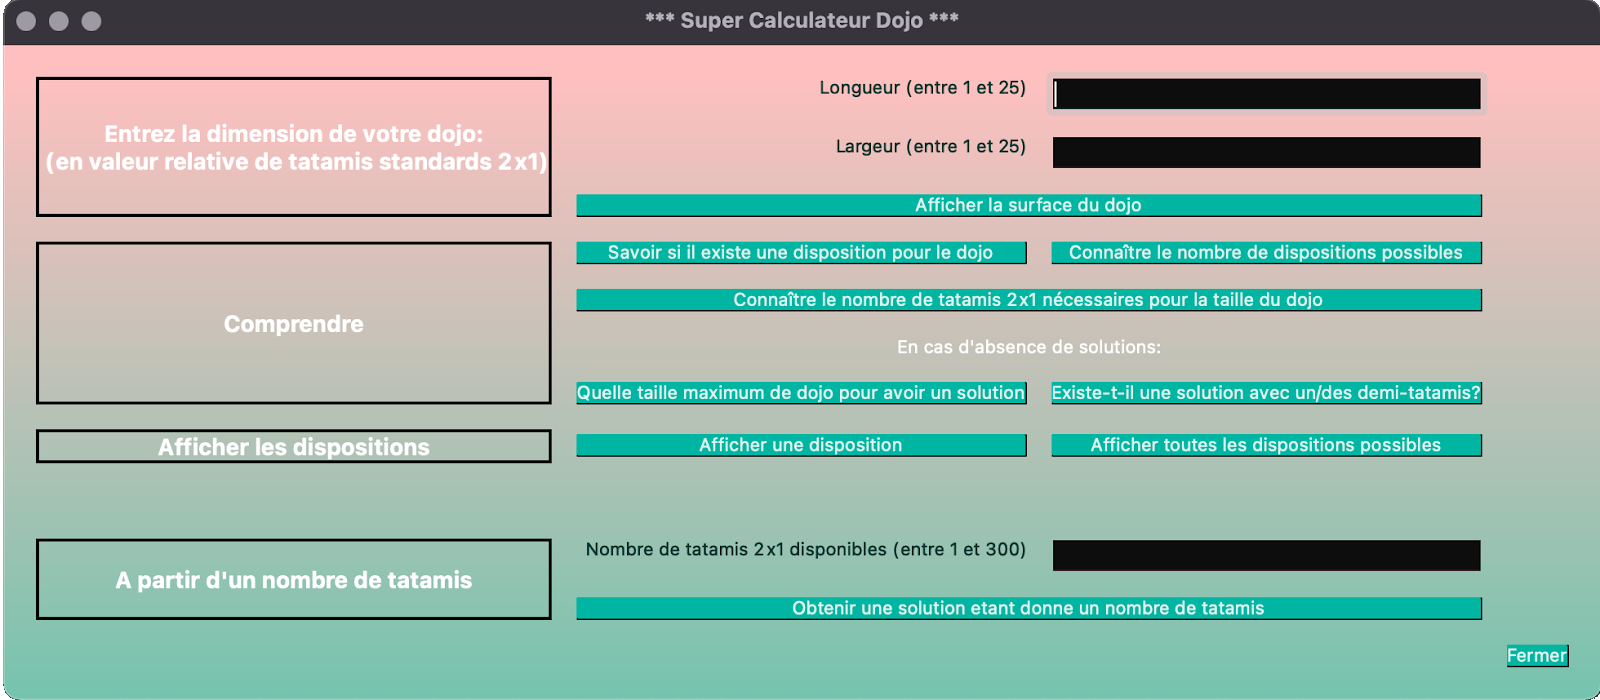
\includegraphics[width=16cm]{images/releaseInterface.png}
\end{center}

\subsection{Choix de la structure du programme}

Dans la continuité de l’application des principes \emph{SOLID}, en particulier la volonté qu’un fichier 
ait une fonction principale, un fichier supplémentaire a été créé \texttt{release.py}. 
L’objectif de ce fichier est d'héberger les fonctionnalités implémentées spécifiquement pour 
cette version, à savoir :
\begin{itemize}
    \item le calcul de solutions pour des dimensions plus petites en cas d’impossibilité de 
    pavage avec les premières dimensions fournies par l’utilisateur.
    \item la fonction de calcul permettant de connaître les dimensions possibles de dojos 
    pour un nombre de tatamis donné.
\end{itemize}

\section{Challenges rencontrés et apprentissage}

\subsection{Challenges rencontrés et solutions appliquées}

Les deux challenges principaux de cette version ont été les suivants:
\begin{itemize}
    \item Charge de travail du sprint. Malgré avoir réalisé lors du précédent Sprint 
    l’importance de ne pas sous-estimer la charge de travail pour un sprint, nous avons eu 
    une nouvelle fois des difficultés dans cet exercice. Nous avons pourtant essayé de bien 
    planifiée (cf. partie suivante ‘Apprentissage’) mais avec 4 fonctionnalités et des travaux 
    sur l’interface, nous avons encore une fois été très ambitieux. La raison est en particulier 
    due au fait que 2 des fonctionnalités ont nécessité des efforts importants sur l'algorithme.
    \item Challenges techniques pour les fonctionnalités:
    \begin{itemize}
        \item Taille maximum d’un dojo ayant des disposition(s) possible(s) (en cas d’absence 
        de solution pour le dojo aux dimensions saisies par l’utilisateur)
        \item Obtention de dimensions de dojos (avec solutions) étant donné un nombre de tatamis 
        saisis par l’utilisateur. Cette fonctionnalité a été particulièrement difficile car les 
        possibilités sont multiples et des critères de sélection ont dû être ajoutés. Une recherche 
        de doublons a également dû être appliquée.
    \end{itemize}
\end{itemize}

\subsection{Apprentissage}

Le principal apprentissage est la phase de préparation et priorisation des User Stories 
à \emph{embarquer} dans la version.

Étant donné les challenges rencontrés lors du précédent Sprint, nous avons décidé de mieux planifier 
les 2 derniers Sprint et avons procédé ainsi:
\begin{itemize}
    \item Liste des fonctionnalités/User stories potentielles
    \item Travaux de recherche et estimation de la complexité selon 2 dimensions: effort sur 
    l'algorithme et effort sur l’interface. Efforts dimensionnés en 3 catégories: faible, moyen et élevé
    \item Décisions sur les User stories pour les 2 derniers Sprint en essayant d'équilibrer la charge de travail.
\end{itemize}
Bien que nous ayons à nouveau sur-dimensionné le Sprint Release Candidate, nous sommes satisfait 
de la méthodologie de planification appliquée. Notre erreur se trouve au niveau de l’estimation 
de l’effort, probablement dû à notre manque d'expérience de la programmation. Pour le dernier Sprint, 
nous essayerons de compenser notre manque d'expérience par une réflexion plus approfondie du travail 
à effectuer pour achever la User Story.

